\chapter{ Testes }

Neste capítulo são apresentados os testes realizados no sistema proposto, integrando o classificador Haar ao codificador do H.264. Testes detalhados de desempenho comparando o classificador Haar do OpenCV com outros 2 algoritmos de detecção de objetos, podem ser vistos em \cite{haarTests}. Todos os testes utilizaram o mesmo arquivo de treinamento \textit{haarcascade\_frontalface\_alt.xml}, que realiza a busca de faces frontais, este arquivo vem junto com a distribuição do OpenCV (que pode ser encontrada em http://sourceforge.net/projects/opencvlibrary/files) no diretório \textit{data/haarcascades}. O tamanho mínimo do objeto de interesse configurado em todos os testes foi de 30 x 30 pixels.

A configuração da máquina e o sistema operacional utilizados nos testes foi:


\begin{itemize}
        \item Processador Pentium(R) Dual-Core E5200 á 2.50GHz.
        \item 4 gigabytes de memória RAM.
        \item Sistema operacional Ubuntu 11.04 32 bits.
\end{itemize}


Os parâmetros medidos foram os seguintes:

\begin{itemize}
        \item Desempenho do sistema com \textit{tracking} de objetos X sem \textit{tracking} de objetos.
	\item Desempenho do sistema com o uso de histerese X sem o uso de histerese.
        \item Desempenho do sistema com diferentes configurações de histerese.
	\item Qualidade do \textit{tracking} de objetos em suas diferentes configurações, constatando visualmente a caixa delimitadora desenhada no vídeo.
	\item Tamanho do bitstream com \textit{tracking} de objetos X sem \textit{tracking} de objetos.
\end{itemize}


Foram realizados 5 testes em cada vídeo:


\begin{itemize}
        \item Sem \textit{tracking} de objetos.

	\item Com \textit{tracking} ativado, com histerese de busca = 1 e histerese de \textit{tracking} = 1. Dessa maneira as informações de estimativa de movimento do codificador não são utilizadas, o \textit{tracking} é realizado utilizando apenas o classificador Haar.

	\item Com \textit{tracking} ativado, com histerese de busca = 5 e histerese de \textit{tracking} = 10. Essa configuração faz um menor uso das informações de estimativa de movimento para realizar \textit{tracking} de um objeto.

         \item Com \textit{tracking} ativado, com histerese de busca = 10 e histerese de \textit{tracking} = 30. Essa configuração depende mais das informações de estimativa de movimento para realizar \textit{tracking} de um objeto.

         \item Com \textit{tracking} ativado, com histerese de busca = 10 e histerese de \textit{tracking} = 60. Essa configuração é a que mais depende mais das informações de estimativa de movimento para realizar \textit{tracking} de um objeto.
\end{itemize}


Dessa maneira é possível avaliar a diferença entre realizar o \textit{tracking} de um objeto utilizando apenas o classificador Haar, ou utilizando histereses com auxílio das informações de estimativa de movimento. Em todos os testes foi utilizada a mesma configuração de codificação, a única diferença entre as configurações são o arquivo de origem, arquivo de destino, resolução e taxa de apresentação (pois esses parâmetros são diferentes para cada vídeo). No apêndice E encontram-se as configurações que foram alteradas a partir do arquivo de configuração original que vem junto com o software de referência (o arquivo de configuração original se encontra em \textit{bin/encoder.cfg}).


\section{ Vídeo Akiyo - QCIF - 300 quadros }


Esse vídeo pode ser encontrado em http://media.xiph.org/video/derf/y4m/akiyo\_qcif.y4m e consiste basicamente de 300 quadros positivos (existe o objeto de interesse ao longo de todo o vídeo, nesse caso uma face frontal).


Especificações do vídeo:

\begin{itemize}
        \item quadros por segundo = 29.97.
        \item total de quadros    = 300.
        \item comprimento         = 176 pixels.
        \item altura              = 144 pixels.
        \item espaço de cor       = YUV, 4:2:0.
\end{itemize}


\begin{table}[H]
\begin{center}
\begin{tabular}{|p{2.3cm}|p{2.3cm}|p{2.3cm}|p{2.3cm}|p{2.3cm}|p{2.3cm}|}
\hline
\textbf{} & \textbf{\textit{Tracking} Desabilitado} & \textbf{\textit{Tracking} habilitado, sem histerese} & \textbf{Histerese de busca = 5, \textit{tracking} = 10} & \textbf{Histerese de busca = 10, \textit{tracking} = 30} & \textbf{Histerese de busca = 10, \textit{tracking} = 60} \\
\hline
Tempo Total de Codificação (segundos) & 35,053 & 38,889 & 35,500 & 35,260 & 35,190 \\
\hline
Tamanho bitstream (bytes) & 359220 & 372974 & 372790 & 372560 & 372561 \\
\hline
Atraso no tempo total codificação & 0\% & 10,94\% & 1,27\% & 0,59\% & 0,39\% \\
\hline
Aumento bitstream  & 0\% & 3,83\% & 3,77\% & 3,71\% & 3,71\% \\
\hline
\end{tabular}
\caption{Desempenho do sistema com o vídeo Akiyo.}
\label{tab:space_overhead}
\end{center}
\end{table}

\begin{figure}[H]
\centering
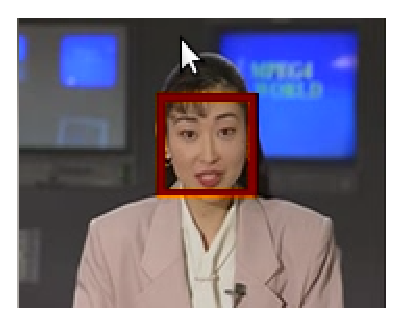
\includegraphics[scale=0.8]{imagens/fig20.eps}
\caption{Face detectada no vídeo Akiyo.}
\label{fig:akiyo_example}
\end{figure}

Como este vídeo é composto de apenas uma pessoa, realizando pequenos movimentos suaves, os resultados com histerese de \textit{tracking} alta foram bons. A ativação de detecção de objetos em todos os quadros, utilizando apenas o classificador Haar para realizar o \textit{tracking}, tornou o processo de codificação aproximadamente 10,94\% mais lento. 

A utilização do classificador Haar em conjunto com a estimativa de movimento fez com que a caixa delimitadora realizasse movimentos mais suaves, com um atraso variando de 1,27\% á 0,39\% em relação ao processo de codificação original, dependendo da configuração da histerese. O aumento no bitstream no pior caso foi de 3,83\%.

Em todos as configurações a qualidade do vídeo codificado mostrou ser a mesma:

\begin{lstlisting}

Y { PSNR (dB), cSNR (dB), MSE }   : {  41.348,  39.978,   6.53497 }
U { PSNR (dB), cSNR (dB), MSE }   : {  49.603,  49.132,   0.79417 }
V { PSNR (dB), cSNR (dB), MSE }   : {  51.103,  51.031,   0.51284 }

Total bits                        : 2873760 (I 1944040, P 929560, NVB 160) 
Bit rate (kbit/s)  @ 30.00 Hz     : 287.38
Bits to avoid Startcode Emulation : 0 
Bits for parameter sets           : 160 
Bits for filler data              : 0

\end{lstlisting}


\section{ Vídeo \textit{Coast guard} - QCIF - 300 quadros }


Esse vídeo pode ser encontrado em http://media.xiph.org/video/derf/y4m/coastguard\_qcif.y4m e consiste basicamente de 300 quadros negativos (não existe o objeto de interesse ao longo de todo o vídeo). Como a histerese de \textit{tracking} não é utilizada neste teste, a configuração com histerese de busca de 10 quadros e histerese de \textit{tracking} de 60 quadros não será apresentada.


Especificações do vídeo:

\begin{itemize}
        \item quadros por segundo = 29.97.
        \item total de quadros    = 300.
        \item comprimento         = 176 pixels.
        \item altura              = 144 pixels. 
        \item espaço de cor       = YUV, 4:2:0.
\end{itemize}


\begin{table}[H]
\begin{center}
\begin{tabular}{|p{2.3cm}|p{2.3cm}|p{2.3cm}|p{2.3cm}|p{2.3cm}|}
\hline
\textbf{} & \textbf{\textit{Tracking} Desabilitado} & \textbf{\textit{Tracking} habilitado, sem histerese} & \textbf{Histerese de busca = 5, \textit{tracking} = 10} & \textbf{Histerese de busca = 10, \textit{tracking} = 30}  \\
\hline
Tempo Total de Codificação (segundos) & 78,200 & 84,800 & 79,482 & 78,896  \\
\hline
Tamanho bitstream (bytes) & 1240200 & 1240200 & 1240200 & 1240200  \\
\hline
Atraso no tempo total codificação & 0\% & 8,43\% & 1,63\% & 0,89\%  \\
\hline
Aumento bitstream  & 0\% & 0\% & 0\% & 0\%  \\
\hline
\end{tabular}
\caption{Desempenho do sistema com o vídeo Coast Guard.}
\label{tab:space_overhead}
\end{center}
\end{table}


A ativação de detecção de objetos em todos os quadros tornou o processo de codificação aproximadamente 8,43\% mais lento. A utilização do classificador Haar com histerese de busca de 10 quadros gerou bons resultados, um atraso de apenas 0,89\% em relação ao processo de codificação original. Com uma histerese de busca de 5 quadros o atraso dobrou para 1,63\%, ainda sendo um valor bem inferior ao atraso gerado pelo processamento de todos os quadros. Como esse vídeo não possui nenhum objeto de interesse o bitstream teve o mesmo tamanho em todas as configurações, e a histerese de \textit{tracking} não foi nem sequer utilizada.


Em todos as configurações a qualidade do vídeo codificado mostrou ser a mesma:

\begin{lstlisting}

Y { PSNR (dB), cSNR (dB), MSE }   : {  36.174,  34.758,  21.73983 }
U { PSNR (dB), cSNR (dB), MSE }   : {  47.488,  46.834,   1.34807 }
V { PSNR (dB), cSNR (dB), MSE }   : {  49.023,  48.567,   0.90448 }

Total bits                        : 9921600 (I 3033832, P 6887608, NVB 160) 
Bit rate (kbit/s)  @ 29.97 Hz     : 991.17
Bits to avoid Startcode Emulation : 0 
Bits for parameter sets           : 160 
Bits for filler data              : 0 

\end{lstlisting}



\section{ Vídeo \textit{Crew} - CIF - 300 quadros }


Esse vídeo pode ser encontrado em http://media.xiph.org/video/derf/y4m/crew\_cif.y4m, possui várias pessoas andando juntas, possuindo diversas faces frontais em uma boa parte do vídeo, andando na direção da câmera (efeito de \textit{zoom}), até que as faces ficam de perfil.


Especificações do vídeo:

\begin{itemize}
        \item quadros por segundo = 29.97.
        \item total de quadros    = 300.
        \item comprimento         = 352 pixels.
        \item altura              = 288 pixels.
        \item espaço de cor       = YUV, 4:2:0.
\end{itemize}


\begin{table}[H]
\begin{center}
\begin{tabular}{|p{2.3cm}|p{2.3cm}|p{2.3cm}|p{2.3cm}|p{2.3cm}|p{2.3cm}|}
\hline
\textbf{} & \textbf{\textit{Tracking} Desabilitado} & \textbf{\textit{Tracking} habilitado, sem histerese} & \textbf{Histerese de busca = 5, \textit{tracking} = 10} & \textbf{Histerese de busca = 10, \textit{tracking} = 30} & \textbf{Histerese de busca = 10, \textit{tracking} = 60} \\
\hline
Tempo Total de Codificação (segundos) & 341,362 & 371,870 & 344,997 & 342,596 & 342,376 \\
\hline
Tamanho bitstream (bytes) & 1245195 & 1255323 & 1256008 & 1256661 & 1257621 \\
\hline
Atraso no tempo total codificação & 0\% & 8,93\% & 1,06\% & 0,36\% & 0,29\% \\
\hline
Aumento bitstream  & 0\% & 0,81\% & 0,86\% & 0,92\% & 0,99\% \\
\hline
\end{tabular}
\caption{Desempenho do sistema com o vídeo Crew.}
\label{tab:space_overhead}
\end{center}
\end{table}


\begin{figure}[H]
\centering
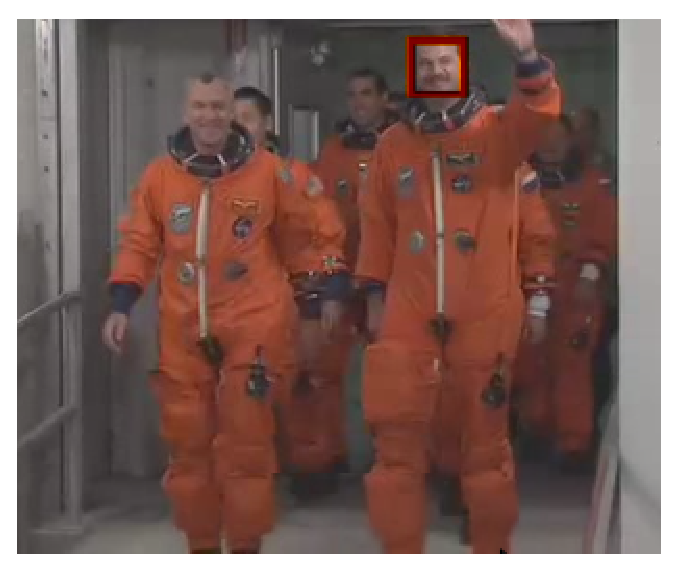
\includegraphics[scale=0.6]{imagens/fig22.eps}
\caption{Face detectada no vídeo \textit{Crew}.}
\label{fig:crew_example}
\end{figure}


Como este vídeo é composto de várias pessoas andando juntas, possui diversas faces frontais simultaneamente. Dessa maneira ele exibe duas limitações do sistema, a capacidade de detectar e realizar o tracking de apenas um objeto por vez (é possível realizar o \textit{tracking} de vários objetos diferentes, utilizando extratores com treinamentos diferentes, mas não o \textit{tracking} de vários objetos com mesma forma), e algumas falhas quando um objeto se move rápido demais (a caixa delimitadora se move mais lentamente que o objeto). 

Quanto ao desempenho a ativação de detecção de objetos em todos os quadros tornou o processo de codificação 8,93\% mais lento. A utilização do classificador Haar em conjunto com a estimativa de movimento diminui consideravelmente o custo computacional, com um atraso no processo de codificação variando entre 1,06\% e 0,29\% em relação ao processo de codificação original. O bitstream com os metadados inseridos no pior caso ficou 0,99\% maior que o bitstream original.


Em todos as configurações a qualidade do vídeo codificado mostrou ser a mesma:

\begin{lstlisting}
Y { PSNR (dB), cSNR (dB), MSE }   : {  35.790,  35.087,  20.15370 }
U { PSNR (dB), cSNR (dB), MSE }   : {  39.443,  38.836,   8.50048 }
V { PSNR (dB), cSNR (dB), MSE }   : {  38.490,  37.766,  10.87730 }

Total bits                        : 10000072 (I 2404808, P 7595096, NVB 168) 
Bit rate (kbit/s)  @ 30.00 Hz     : 1000.01
Bits to avoid Startcode Emulation : 0 
Bits for parameter sets           : 168 
Bits for filler data              : 0
\end{lstlisting}


\section{ Vídeo Foreman - CIF - 300 quadros }


Esse vídeo pode ser encontrado em http://media.xiph.org/video/derf/y4m/foreman\_cif.y4m e possui 3 situações diferentes, uma face frontal, a face fica de perfil em alguns momentos, e depois a face sai do vídeo.


Especificações do vídeo:

\begin{itemize}
        \item quadros por segundo = 29.97.
        \item total de quadros    = 300.
        \item comprimento         = 352 pixels.
        \item altura              = 288 pixels.
        \item espaço de cor       = YUV, 4:2:0.
\end{itemize}


\begin{table}[H]
\begin{center}
\begin{tabular}{|p{2.3cm}|p{2.3cm}|p{2.3cm}|p{2.3cm}|p{2.3cm}|p{2.3cm}|}
\hline
\textbf{} & \textbf{\textit{Tracking} Desabilitado} & \textbf{\textit{Tracking} habilitado, sem histerese} & \textbf{Histerese de busca = 5, \textit{tracking} = 10} & \textbf{Histerese de busca = 10, \textit{tracking} = 30} & \textbf{Histerese de busca = 10, \textit{tracking} = 60} \\
\hline
Tempo Total de Codificação (segundos) & 260,432 & 286,162 & 265,003 & 262,654 & 262,126 \\
\hline
Tamanho bitstream (bytes) & 1244893 & 1249485 & 1250345 & 1251793 & 1253161 \\
\hline
Atraso no tempo total codificação & 0\% & 9,87\% & 1,75\% & 0,85\% & 0,65\% \\
\hline
Aumento bitstream  & 0\% & 0,36\% & 0,43\% & 0,55\% & 0,66\% \\
\hline
\end{tabular}
\caption{Desempenho do sistema com o vídeo Foreman.}
\label{tab:space_overhead}
\end{center}
\end{table}

\begin{figure}[H]
\centering
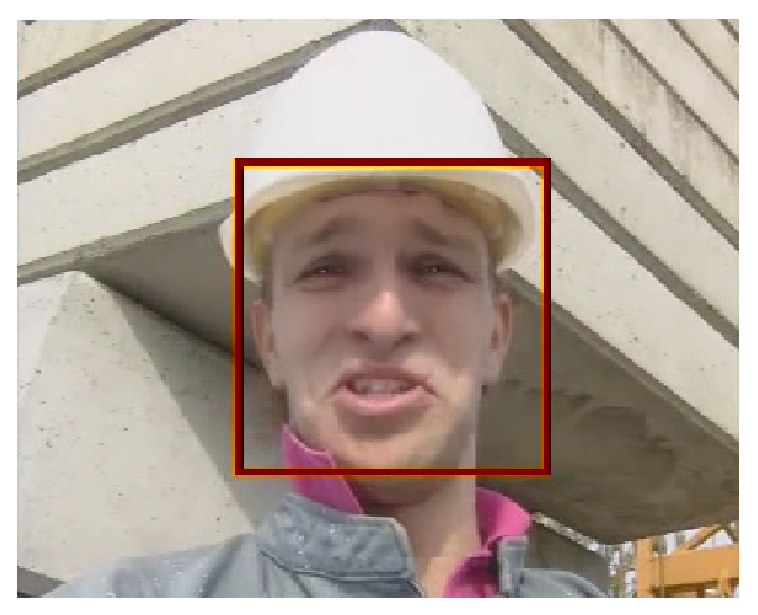
\includegraphics[scale=0.6]{imagens/fig21.eps}
\caption{Face detectada no vídeo Foreman.}
\label{fig:foreman_example}
\end{figure}

Com a detecção de objetos ocorrendo em todos os quadros percebe-se uma alta taxa de falsos negativos, já que o rosto no vídeo fica de perfil em alguns momentos e o classificador Haar não consegue identificar o rosto em perfil, perdendo assim o \textit{tracking} do rosto. Com a detecção de objetos em todos os quadros também ocorreu um falso positivo quando a câmera se move e deixa de gravar o rosto. A medida que a histerese de \textit{tracking} é aumentada, além de não ocorrer o falso positivo, os movimentos que o rosto realiza são acompanhados com maior suavidade e com uma menor taxa de falsos negativo (com a histerese de \textit{tracking} configurada para 60 quadros não ocorreu nenhum falso negativo). 

Quanto ao desempenho a ativação de detecção de objetos em todos os quadros tornou o processo de codificação 9,87\% mais lento. A utilização do classificador Haar em conjunto com a estimativa de movimento diminui consideravelmente o custo computacional, com um atraso no processo de codificação variando entre 1,75\% e 0,65\% em relação ao processo de codificação original. O bitstream com os metadados inseridos no pior caso ficou 0,66\% maior que o bitstream original.


Em todos as configurações a qualidade do vídeo codificado mostrou ser a mesma:

\begin{lstlisting}
Y { PSNR (dB), cSNR (dB), MSE }   : {  36.017,  34.568,  22.71311 }
U { PSNR (dB), cSNR (dB), MSE }   : {  41.277,  40.985,   5.18274 }
V { PSNR (dB), cSNR (dB), MSE }   : {  43.175,  42.592,   3.57977 }

Total bits                        : 9959144 (I 2813168, P 7145808, NVB 168) 
Bit rate (kbit/s)  @ 30.00 Hz     : 995.91
Bits to avoid Startcode Emulation : 0 
Bits for parameter sets           : 168 
Bits for filler data              : 0
\end{lstlisting}


\section{ Vídeo \textit{Pedestrian area} - 375 quadros }


Esse vídeo pode ser encontrado em http://media.xiph.org/video/derf/y4m/pedestrian\_area\_1080p25.y4m. Ele consiste basicamente de vários pedestres caminhando em uma rua, possui faces frontais e faces em perfil se movendo continuamente. 


\subsection{ Testes com resolução 1080p (1920 x 1080) }

Especificações do vídeo:

\begin{itemize}
        \item quadros por segundo = 25.
        \item total de quadros    = 375.
        \item comprimento         = 1920 pixels.
        \item altura              = 1080 pixels.
        \item espaço de cor       = YUV, 4:2:0.
\end{itemize}


\begin{table}[H]
\begin{center}
\begin{tabular}{|p{2.3cm}|p{2.3cm}|p{2.3cm}|p{2.3cm}|p{2.3cm}|p{2.3cm}|}
\hline
\textbf{} & \textbf{\textit{Tracking} Desabilitado} & \textbf{\textit{Tracking} habilitado, sem histerese} & \textbf{Histerese de busca = 5, \textit{tracking} = 10} & \textbf{Histerese de busca = 10, \textit{tracking} = 30} & \textbf{Histerese de busca = 10, \textit{tracking} = 60} \\
\hline
Tempo Total de Codificação (segundos) & 6915.861 & 7280.818 & 6921.871 & 6918.653 & 6916.272 \\
\hline
Tamanho bitstream (bytes) & 7854045 & 7870345 & 7870468 & 7870642 & 7870601 \\
\hline
Atraso no tempo total codificação & 0\% & 5,27\% & 0,08\% & 0,04\% & 0,005\% \\
\hline
Aumento bitstream  & 0\% & 0,207\% & 0,209\% & 0,211\% & 0,210\% \\
\hline
\end{tabular}
\caption{Desempenho do sistema com o vídeo \textit{Pedestrian area}.}
\label{tab:space_overhead}
\end{center}
\end{table}

\begin{figure}[H]
\centering
\includegraphics[scale=0.3]{imagens/fig25.eps}
\caption{Face detectada no vídeo \textit{Pedestrian area}.}
\label{fig:pedestrian_example}
\end{figure}

Com a detecção de objetos ocorrendo em todos os quadros ocorre uma grande quantidade de falsos positivos, e a limitação de realizar o \textit{tracking} de apenas um objeto por vez ficou bem evidente já que neste vídeo existem diversas pessoas andando ao mesmo tempo o sistema consegue realizar o \textit{tracking} de algumas faces por um curto período de tempo, mas logo depois detecta outra face e passa a realizar o \textit{tracking} dessa face ao invés da que foi previamente detectada. 

A utilização das histereses alterou um pouco o comportamento do sistema (em geral ele manteve uma alta taxa de falsos positivos), a primeira detecção que ocorre com sucesso realiza o \textit{tracking} da face corretamente, mas após essa primeira detecção ocorre uma série de falsos positivos, e em algumas detecções positivas o \textit{tracking} não consegue acompanhar a face por ela estar se movendo rápido demais.

Quanto ao desempenho a ativação de detecção de objetos em todos os quadros tornou o processo de codificação 5,27\% mais lento. A utilização do classificador Haar em conjunto com a estimativa de movimento diminui consideravelmente o custo computacional, com um atraso no processo de codificação inferior a 0,1\% em todas as configurações de histerese testadas. O bitstream com os metadados inseridos no pior caso ficou 0,211\% maior que o bitstream original.


Em todos as configurações a qualidade do vídeo codificado mostrou ser a mesma:

\begin{lstlisting}
Y { PSNR (dB), cSNR (dB), MSE }   : {  37.196,  37.136,  12.57412 }
U { PSNR (dB), cSNR (dB), MSE }   : {  41.390,  41.356,   4.75815 }
V { PSNR (dB), cSNR (dB), MSE }   : {  42.574,  42.530,   3.63104 }

Total bits                        : 62832360 (I 11049512, P 51782664, NVB 184) 
Bit rate (kbit/s)  @ 25.00 Hz     : 4188.82
Bits to avoid Startcode Emulation : 0 
Bits for parameter sets           : 184 
Bits for filler data              : 0
\end{lstlisting}


\subsection{ Testes com resolução 720p (1280 x 720) }


Neste teste a resolução do vídeo que foi reduzida de \textit{1080p} (1920 x 1080) para \textit{720p} (1280 x 720), visando a constatação da diferença do impacto do sistema de \textit{tracking} ao processar o mesmo vídeo com resoluções diferentes. O escalonamento do vídeo foi realizado utilizando o Gstreamer.


Especificações do vídeo:

\begin{itemize}
        \item quadros por segundo = 25.
        \item total de quadros    = 375.
        \item comprimento         = 1280 pixels.
        \item altura              = 720 pixels.
        \item espaço de cor       = YUV, 4:2:0.
\end{itemize}


\begin{table}[H]
\begin{center}
\begin{tabular}{|p{2.3cm}|p{2.3cm}|p{2.3cm}|p{2.3cm}|p{2.3cm}|p{2.3cm}|}
\hline
\textbf{} & \textbf{\textit{Tracking} Desabilitado} & \textbf{\textit{Tracking} habilitado, sem histerese} & \textbf{Histerese de busca = 5, \textit{tracking} = 10} & \textbf{Histerese de busca = 10, \textit{tracking} = 30} & \textbf{Histerese de busca = 10, \textit{tracking} = 60} \\
\hline
Tempo Total de Codificação (segundos) & 2986.361 & 3317.612 & 3011.626 & 2999.675 & 2993.329 \\
\hline
Tamanho bitstream (bytes) & 4269076 & 4283747 & 4284989 & 4283815 & 4284129 \\
\hline
Atraso no tempo total codificação & 0\% & 11,09\% & 0,84\% & 0,44\% & 0,23\% \\
\hline
Aumento bitstream  & 0\% & 0,34\% & 0,37\% & 0,34\% & 0,35\% \\
\hline
\end{tabular}
\caption{Desempenho do sistema com o vídeo \textit{Pedestrian area - 720p}.}
\label{tab:space_overhead}
\end{center}
\end{table}

A diminuição da resolução do vídeo não gerou nenhuma diferença na qualidade do \textit{tracking}, porém foi possível perceber um aumento no atraso no tempo total de codificação em todas as configurações. Com \textit{tracking} habilitado e sem histerese, o atraso no vídeo original (\textit{1080p}) foi de 5,27\% enquanto que o atraso gerado no mesmo vídeo, reescalonado para \textit{720p}, foi de 11,09\%, mostrando que a medida que o tamanho do vídeo aumenta o atraso gerado pelo classificador Haar tende a diminuir.

Em todos as configurações a qualidade do vídeo codificado mostrou ser a mesma:

\begin{lstlisting}
Y { PSNR (dB), cSNR (dB), MSE }   : {  36.269,  36.196,  15.61449 }
U { PSNR (dB), cSNR (dB), MSE }   : {  40.982,  40.944,   5.23199 }
V { PSNR (dB), cSNR (dB), MSE }   : {  41.777,  41.730,   4.36622 }

Total bits                        : 34152608 (I 6300464, P 27851968, NVB 176) 
Bit rate (kbit/s)  @ 25.00 Hz     : 2276.84
Bits to avoid Startcode Emulation : 0 
Bits for parameter sets           : 176 
Bits for filler data              : 0 
\end{lstlisting}


\section{ Vídeo \textit{Speed bag} - 570 quadros }


Esse vídeo pode ser encontrado em http://media.xiph.org/video/derf/y4m/speed\_bag\_1080p.y4m. Uma parte do vídeo possui uma face frontal realizando pequenos movimentos. O vídeo original se encontra com espaço de cor YUV 4:2:2, porém para facilitar o procedimento de teste e a comparação com os resultados de outros vídeos ele foi convertido para o espaço de cor YUV 4:2:0, utilizando o Gstreamer. O vídeo consiste de um face de perfil se movendo (pessoa caminhando), nenhuma face, uma face frontal realizando movimentos suaves e depois uma face de perfil realizando movimentos rápidos (pugilista socando um saco de pancada).


\subsection{ Testes com resolução 1080p (1920 x 1080) }

Especificações do vídeo:

\begin{itemize}
        \item quadros por segundo = 29.97.
        \item total de quadros    = 570.
        \item comprimento         = 1920 pixels.
        \item altura              = 1080 pixels.
        \item espaço de cor       = YUV, 4:2:0.
\end{itemize}


\begin{table}[H]
\begin{center}
\begin{tabular}{|p{2.3cm}|p{2.3cm}|p{2.3cm}|p{2.3cm}|p{2.3cm}|p{2.3cm}|}
\hline
\textbf{} & \textbf{\textit{Tracking} Desabilitado} & \textbf{\textit{Tracking} habilitado, sem histerese} & \textbf{Histerese de busca = 5, \textit{tracking} = 10} & \textbf{Histerese de busca = 10, \textit{tracking} = 30} & \textbf{Histerese de busca = 10, \textit{tracking} = 60} \\
\hline
Tempo Total de Codificação (segundos) & 12719.172 & 13689.180 & 12867.480 & 12821.436 & 12765.063 \\
\hline
Tamanho bitstream (bytes) & 8409840 & 8425882 & 8428471 & 8428672 & 8430918 \\
\hline
Atraso no tempo total codificação & 0\% & 7,62\% & 1,16\% & 0,8\% & 0,36\% \\
\hline
Aumento bitstream  & 0\% & 0,19\% & 0,22\% & 0,22\% & 0,25\% \\
\hline
\end{tabular}
\caption{Desempenho do sistema com o vídeo \textit{Speed bag - 1080p}.}
\label{tab:space_overhead}
\end{center}
\end{table}

\begin{figure}[H]
\centering
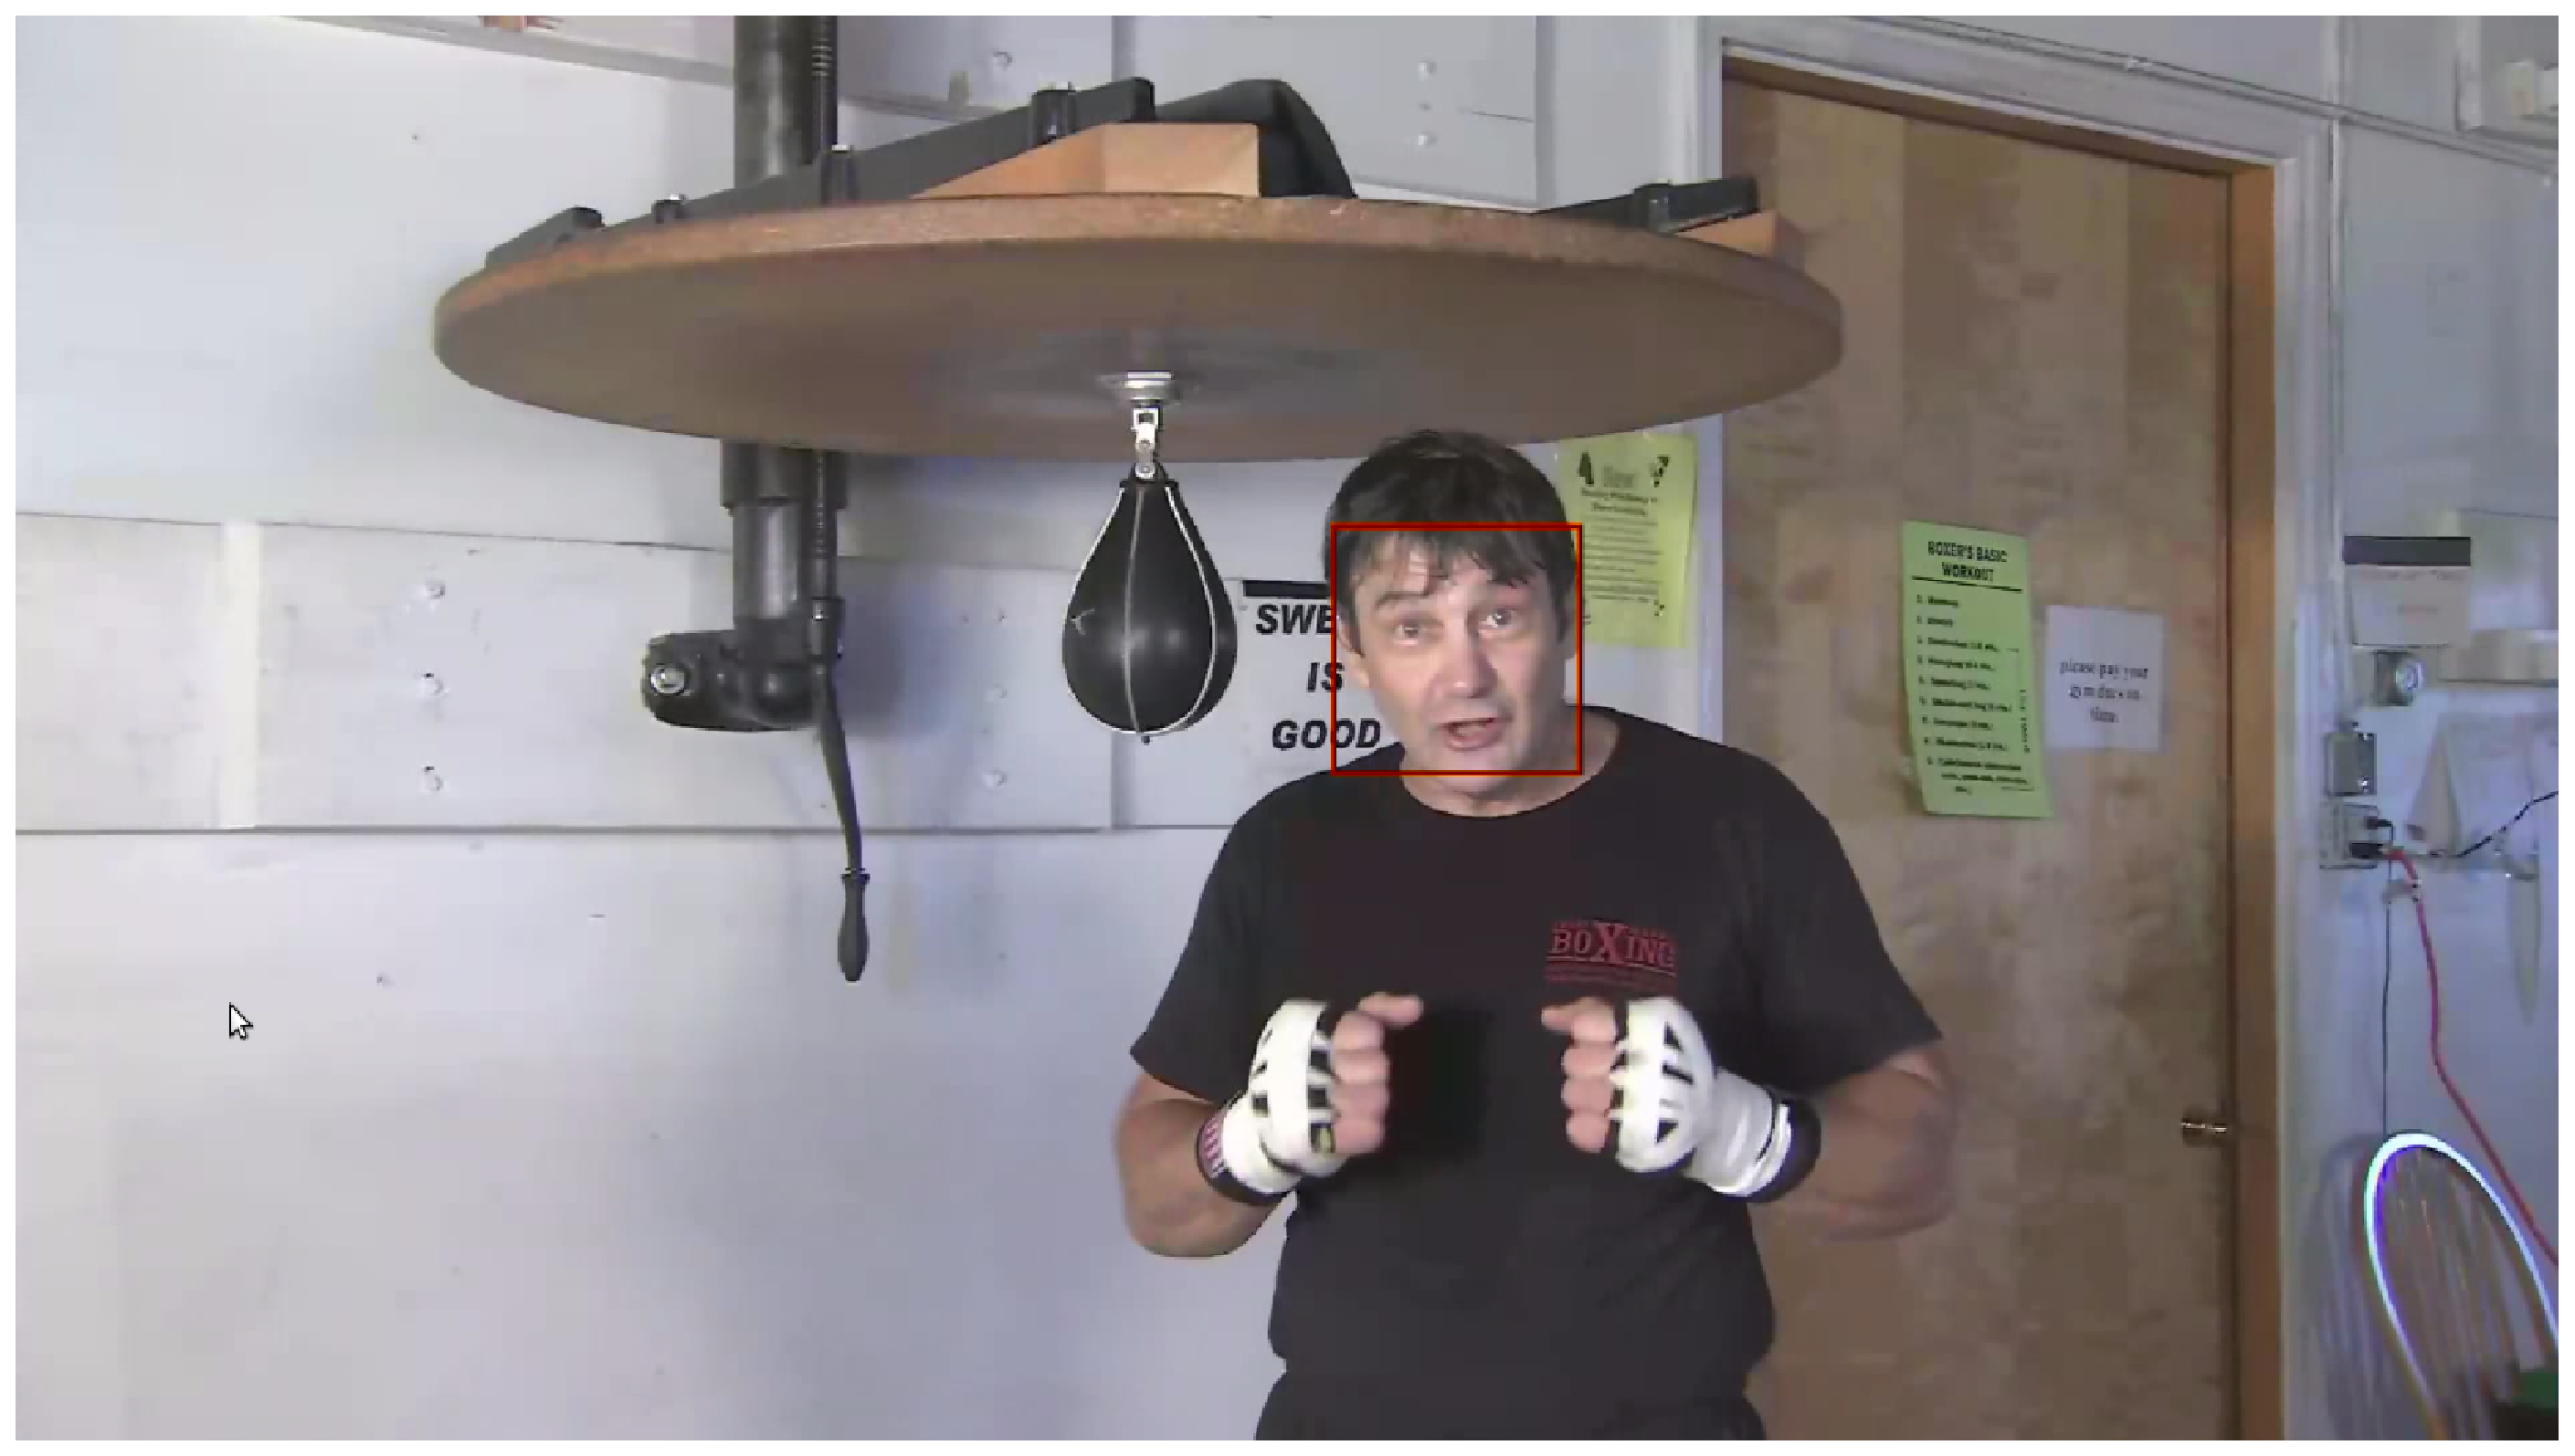
\includegraphics[scale=0.3]{imagens/fig26.eps}
\caption{Face detectada no vídeo \textit{Speed bag}.}
\label{fig:speed_bag_example}
\end{figure}

Utilizando a detecção de objetos em todos os quadros ocorrem diversos falsos positivos, a maior parte dos momentos em que existe a face de perfil ocorrem falsos positivos ou falsos negativos. O momento em que ocorre a face frontal no vídeo possui uma maior quantidade de positivos, porém em alguns momentos ocorrem falsos positivos (um objeto no fundo é detectado como a face), mostrando claramente a limitação que existe ao se configurar o classificador Haar para realizar a detecção de apenas um objeto na imagem. O \textit{tracking} pode se confundir ao detectar outro objeto que não é uma face, já que apenas o primeiro objeto a ser encontrado na imagem é retornado pelo classificador Haar. 

A utilização de histereses ofereceu pouca melhora na qualidade do \textit{tracking}, já que neste vídeo a quantidade de falsos positivos foi muito grande. Apenas no momento em que ocorria a face frontal a histerese mostrou uma melhora significativa, já que a face frontal era detectada e durante a histerese de \textit{tracking} apenas os vetores de movimento calculados pela estimativa de movimento era utilizados para realizar o \textit{tracking}, reduzindo os falsos positivos gerados pelo classificador Haar.

Quanto ao desempenho a ativação de detecção de objetos em todos os quadros tornou o processo de codificação 7,62\% mais lento. A utilização do classificador Haar em conjunto com a estimativa de movimento diminui consideravelmente o custo computacional, com um atraso no processo de codificação variando entre 1,16\% e 0,36\% em relação ao processo de codificação original. O bitstream com os metadados inseridos no pior caso ficou 0,25\% maior que o bitstream original.


Em todos as configurações a qualidade do vídeo codificado mostrou ser a mesma:

\begin{lstlisting}
Y { PSNR (dB), cSNR (dB), MSE }   : {  39.554,  39.283,   7.67013 }
U { PSNR (dB), cSNR (dB), MSE }   : {  43.495,  43.394,   2.97618 }
V { PSNR (dB), cSNR (dB), MSE }   : {  44.830,  44.669,   2.21926 }

Total bits                        : 67278720 (I 9809312, P 57469224, NVB 184) 
Bit rate (kbit/s)  @ 30.00 Hz     : 3540.99
Bits to avoid Startcode Emulation : 0 
Bits for parameter sets           : 184 
Bits for filler data              : 0
\end{lstlisting}


\subsection{ Testes com resolução 720p (1280 x 720) }


Neste teste a resolução do vídeo que foi reduzida de \textit{1080p} (1920 x 1080) para \textit{720p} (1280 x 720), visando a constatação da diferença do impacto do sistema de \textit{tracking} ao processar o mesmo vídeo a resoluções diferentes. O escalonamento do vídeo foi realizado utilizando o Gstreamer.


Especificações do vídeo:

\begin{itemize}
        \item quadros por segundo = 29.97.
        \item total de quadros    = 570.
        \item comprimento         = 1280 pixels.
        \item altura              = 720 pixels.
        \item espaço de cor       = YUV, 4:2:0.
\end{itemize}


\begin{table}[H]
\begin{center}
\begin{tabular}{|p{2.3cm}|p{2.3cm}|p{2.3cm}|p{2.3cm}|p{2.3cm}|p{2.3cm}|}
\hline
\textbf{} & \textbf{\textit{Tracking} Desabilitado} & \textbf{\textit{Tracking} habilitado, sem histerese} & \textbf{Histerese de busca = 5, \textit{tracking} = 10} & \textbf{Histerese de busca = 10, \textit{tracking} = 30} & \textbf{Histerese de busca = 10, \textit{tracking} = 60} \\
\hline
Tempo Total de Codificação (segundos) & 5346.245 & 5843.674 & 5394.242 & 5365.767 & 5352.772 \\
\hline
Tamanho bitstream (bytes) & 4595164 & 4607265 & 4609359 & 4612805 & 4616437 \\
\hline
Atraso no tempo total codificação & 0\% & 9,3\% & 0,89\% & 0,36\% & 0,12\% \\
\hline
Aumento bitstream  & 0\% & 0,26\% & 0,30\% & 0,38\% & 0,46\% \\
\hline
\end{tabular}
\caption{Desempenho do sistema com o vídeo \textit{Speed bag - 720p}.}
\label{tab:space_overhead}
\end{center}
\end{table}


A diminuição da resolução do vídeo não gerou nenhuma diferença na qualidade do \textit{tracking}, porém foi possível perceber um aumento no atraso no tempo total de codificação em todas as configurações. Com \textit{tracking} habilitado e sem histerese, o atraso no vídeo original (\textit{1080p}) foi de 7,62\% enquanto que o atraso gerado no mesmo vídeo, reescalonado para \textit{720p}, foi de 9,3\%, mostrando que a medida que o tamanho do vídeo aumenta o atraso gerado pelo classificador Haar tende a diminuir.


Em todos as configurações a qualidade do vídeo codificado mostrou ser a mesma:

\begin{lstlisting}
Y { PSNR (dB), cSNR (dB), MSE }   : {  39.131,  38.752,   8.66746 }
U { PSNR (dB), cSNR (dB), MSE }   : {  43.023,  42.893,   3.34007 }
V { PSNR (dB), cSNR (dB), MSE }   : {  44.422,  44.220,   2.46079 }

Total bits                        : 36761312 (I 5554416, P 31206720, NVB 176) 
Bit rate (kbit/s)  @ 30.00 Hz     : 1934.81
Bits to avoid Startcode Emulation : 0 
Bits for parameter sets           : 176 
Bits for filler data              : 0
\end{lstlisting}


\section{ Conclusão da avaliação do sistema }


De acordo com os testes realizados a utilização de uma histerese na execução do classificador Haar tornou o sistema mais eficiente. Se somente fosse utilizada a histerese, isso geraria saltos na caixa delimitadora, o uso da estimativa de movimento suavizou esse efeito sem aumentar a complexidade do codificador, já que a estimativa de movimento faz parte do processo normal de codificação. Dependendo da natureza do movimento realizado pelo objeto, a utilização da estimativa de movimento pode gerar resultados inferiores ou superiores á execução do classificador Haar em todos os quadros.

Por exemplo, nos testes apresentados o objeto de interesse era face frontal. Sem utilizar a estimativa de movimento quando uma face se vira de lado o classificador Haar não consegue mais detectar a face que está de perfil, porém utilizando estimativa de movimento o tracking da face de perfil funciona já que uma vez identificado o objeto só é necessário acompanhar seus movimentos. Ao mesmo tempo, dependendo do quanto o objeto de interesse se mover a caixa delimitadora não acompanha perfeitamente o movimento do objeto utilizando as informações de estimativa de movimento. 

Em vídeos com longos trechos sem nenhum objeto de interesse o impacto do classificador Haar tende a ser um pouco menor que o normal, mas em conjunto com a histerese de busca o custo computacional foi reduzido. Inserir um metadado por quadro, mesmo onde o vídeo possui o objeto de interesse em grande parte dos seus quadros, não gerou um bitstream muito maior que o normal, o pior caso não passou de um aumento de 4\%, considerando que quanto maior for a resolução do vídeo e a qualidade do processo de codificação, menor será esse aumento em relação ao bitstream original (isso pode ser observado nos testes com diferentes resoluções).

Com relação ao impacto da utilização do classificador Haar integrado ao codificador em diferentes resoluções, foi possível observar que a medida que a resolução do vídeo aumenta, o custo computacional do processo de codificação tende a aumentar mais que o custo computacional do classificador Haar, já que nos testes em vídeos com alta resolução o impacto da utilização do sistema de \textit{tracking} foi menor que nos vídeos com resoluções menores. Esse resultado foi obtido com o perfil de codificação utilizado nos testes, seria interessante realizar testes com outros perfis de codificação, pois poderiam mostrar resultados diferentes.

Percebe-se também a necessidade de realizar a detecção e \textit{tracking} de múltiplos objetos (que sejam do mesmo padrão, ou seja, utilizem o mesmo arquivo de treinamento para realizar a busca) simultaneamente, como pode ser constatado em \cite{learningOpenCV} página 507, o classificador Haar tende a ter uma baixa taxa de falsos negativos (ou seja, não detectar a presença de um objeto de interesse), em troca de ter uma alta taxa de falsos positivos (detectar um objeto que não é o de interesse), por causa disso utilizar o classificador Haar para retornar o primeiro objeto encontrado simplifica o sistema mas deixa o \textit{tracking} mais suscetível a erros.
  
